\documentclass[11pt]{article}

\usepackage{graphicx}
\usepackage{hyperref}
\usepackage{natbib}

\bibliographystyle{plain}  % or unsrt, alpha, etc.
\setlength{\textwidth}{6.5in}
\setlength{\headheight}{0in}
\setlength{\textheight}{8.0in}
\setlength{\hoffset}{0in}
\setlength{\voffset}{0in}
\setlength{\oddsidemargin}{0in}
\setlength{\evensidemargin}{0in}

\title{Computational Physics -  Problem Set 2}
  
\author{Frederik Holst Knudsen}


\begin{document}

\maketitle

\section{IEEE 32-bit Value}
\label{sec:intro}
By extracting the sign, mantissa and the exponent from the 32-bit float value: 100.98763, I compute the actual value by using eq. (2) from the "Intro" notesheet. The actual number is computed to be 100.98763275146484, where the difference between that and the actual value is: 
$2.75146484\times 10^{-6}$.

\section{32-bit vs. 64-bit Precision}
I declare respectively 32 Bit and 64 Bit floats of 1.0 and a subtraction value and let a loop run starting from a very small subtraction value ($1\times10^{-40})$. The loop runs as long as the subtraction is equal to 1.0 and at every iteration the subtraction value is scaled with a factor of 1.0001. 

For 32-Bit precision the smallest possible subtraction value is $2.9803843\times10^{-8}$

For 64-Bit precision the smallest possible subtraction value is $5.551172870064363\times10^{-17}$


Secondly, I find the largest and smallest values that 32-bit and 64-bit floats can take without underflow and overflow. 

I iterate like before with a small scaling at each step of 1.001. Before updating the value, I ask if the float is equal to Inf. If it is, I will print the i-1 value of the iteration.

Maximum value for 32-bit float: $3.4026\times 10^{38}$ 

Maximum values for 64-bit float: $1.7975\times 10^{308}$ 

The minimum values are found in a similar way: 

Minimum value for 32-bit float: $1\times 10^{-45}$ 

Minimum values for 64-bit float: $1\times 10^{-323}$ 


\section{Newman 2.9}
The Madelung constant is computed to be 1.742 (compared to the actual value, 1.747 for L$\to\infty$) with L=100 using three for-loops. Using Timeit, the  time to complete 10 computations is 338.2 seconds. By creating a mesh with np.meshgrid, we sum over the lattice sites which is much faster. This way, it only takes 5.5 seconds to complete 10 computations. Both computations yield the same result. 

\section{Newman 3.7}
\begin{figure}[h!]
    \centering
    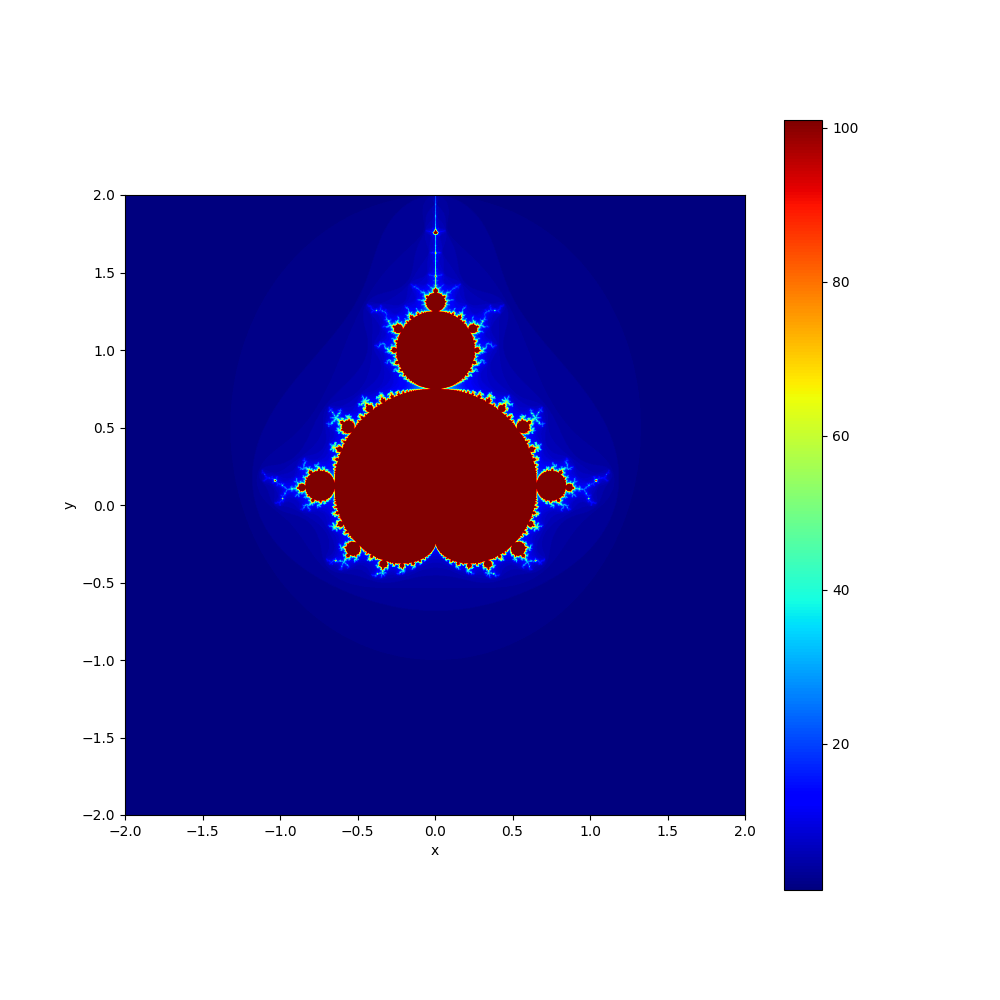
\includegraphics[width=0.7\textwidth]{fractal.png}
    \caption{The Mandelbrot set with maximum iteration number of 100. Heightmap is set so that points that are larger than two, take on the number of iterations before it exceeded this threshold. Points that never exceed the threshold will take the value 101.   }
    \label{fig:your_label}
\end{figure}

\section{Newman 4.2}
The roots using solver 1 are: 

$x_1=-9.999894245993346 \times 10^{-7}$
$x_2=-9.99999999999 \times 10^{5}$

And for solver 2 we have: 
$x_1=-1.000000000001 \times 10^{-6}$
$x_2=-1.0000105755125057\times10^{6}$


From these results we see that the two solvers have different precision for the two different roots. This is due to the increased numerical error when subtracting large, similar numbers. For a better solver, we choose for each root the solver that doesn't deal with subtraction with two numbers have very similar values. After running the test file, we pass both tests.


\end{document}